\documentclass[]{article}
\usepackage{amssymb}
\usepackage{amsmath}
\usepackage[utf8]{inputenc}
\usepackage{graphicx}
\usepackage{booktabs}
\usepackage{listings}
\usepackage{color}
\usepackage{tabularx}
\usepackage{hyperref}

\definecolor{dkgreen}{rgb}{0,0.6,0}
\definecolor{gray}{rgb}{0.5,0.5,0.5}
\definecolor{mauve}{rgb}{0.58,0,0.82}

\lstset{frame=tb,
	%language=C++,
	aboveskip=3mm,
	belowskip=3mm,
	showstringspaces=false,
	columns=flexible,
	basicstyle={\small\ttfamily},
	numbers=none,
	numberstyle=\tiny\color{gray},
	keywordstyle=\color{blue},
	commentstyle=\color{dkgreen},
	stringstyle=\color{mauve},
	breaklines=false,
	breakatwhitespace=true,
	tabsize=2
}


\title{FYS-STK4155 H20 - Project 3:\\Creating a Power Transfomer Cooling System Model using Autoregression and Recurrent Neural Networks}
\author{Olav Fønstelien}

\begin{document}
\maketitle

\begin{abstract}
%The abstract gives the reader a quick overview of what has been done and the most important results. Try to be to the point and state your main findings. It could be structured as follows 
% - Short introduction to topic and why its important 
% - Introduce a challenge or unresolved issue with the topic (that you will try to solve) 
% - What have you done to solve this 
% - Main Results 
% - The implications
This report suggests a power transformer air cooling system model which accurately predicts the winding temperature under dynamic conditions. The model is designed using data collected from a transformer serving an industrial process with highly varying power demand. It consists of two parts; one which predicts the transformer winding temperature based on current and the cooling fan running status; and one which predicts the winding temperature of each winding based on the temperature of the two others. In validation, the predicted temperature deviates from the actual by 1-2 K at the highest load peaks. The model is suggested for condition monitoring of cooling efficiency, as well as detection of sub-optimal cooling of individual windings. The model requires no parametrization and is completely non-intrusive towards the process during implementation and service.

The reports suggest two different implementations of the model; one by autoregression and one by recurrent neural network. The autoregressive model as suggested can easily be employed in industrial environments like programmable logic controllers due to its light weight and simple implementation. The report also reviews the relevant background of both AR and RNN methods, as well as that of air-cooled power transformers.

Please visit my GitHub repository \url{https://github.com/fonstelien/FYS-STK4155/tree/master/project3} for the Python source code developed for this report.
\end{abstract}

\section{Introduction} \label{sec:intro}
%When you write the introduction you could focus on the following aspects
% - Motivate the reader, the first part of the introduction gives always a motivation and tries to give the overarching ideas
% - What I have done
% - The structure of the report, how it is organized etc

% intro to condition monitoring of electric machines
% intro to insulation and temperature
% intro to transformers

Electric machines are highly reliable when properly designed and maintained. They are the workhorses in any industrial process, as well as the actuator in safety-critical functions, and failure may have both economic and physical consequences in the form of production downtime and personnel injury. Ensuring proper function of the machinery is a major cost driver in industry -- dedicated technicians are employed to execute detailed maintenance schedules while others log and monitor performance indicators like temperatures, oil quality and vibration levels. Improving and automating such procedures is a large part of what \textit{Industry 4.0} is about. \textit{Digital twins} of the machines can be used to predict faults which are developing too slowly to be noticed, or which may not even be detectable without the application of advanced data analysis methods. 

Industrial processes introduce complex environments and modeling machine behavior by analytical methods is a highly non-trivial tasks. Statistical and machine learning methods therefore play a central part in the development of digital twins. In this report we will see how a simple model for condition monitoring of the cooling system of an electric power transformer can be created by the use of traditional autoregression and more modern neural networks. Even small increases in a transformer's operating temperature may have severe effects on the lifetime of its electrical insulation, and ensuring that the cooling system performs as designed is vital for the reliability and performance of the transformer. We will create model which lets us evaluate the cooling system's performance under dynamic operating conditions. The model is based only on a few input measurements which are normally monitored in a standard plant automation and control system, and requires no parametrization. The performance at the time of model creation will serve as the baseline against which future performance will be measured.

For developing this model we have available a dataset containing operational data of a power transformer -- an introduction of which is given further down in Section \ref{sec:case-description}. In Section \ref{sec:methods} we will investigate three different approaches to creating the cooling system model; one physical, where we exploit what we know about heat transfer and electric power losses in a conductor; then an autoregressive approach, where we carry over our insights from the physical approach to design input variables in an AR model. At last we investigate an approach using recurrent neural networks. The results are presented in Section \ref{sec:results}, where we go through how each part of the model performs with each of the approaches. Here, we will pay special attention to the \textit{positive} temperature peaks. The report ends by summing up our findings and putting them into an industrial context in Section \ref{sec:conclusion}, where we will also give some thoughts on further expansions and the model's utility in similar applications. But first; power transformer essentials.

\section{Background: Power Transformers and the Case in Study}
In this section we will review the basics that we need to know about power transformers for this report and introduce the technical terminology. We will also give a short description of the case in study and show how the transformer is operated.

\subsection{Electric Power Transformer Basics} \label{sec:transformers}
Electrical power distribution networks usually have several voltage levels, and it is the power transformer's job to \textit{transform} the power from one voltage level to another. In a three-phase power system, each phase will be connected to separate transformer \textit{windings} -- one per phase for the high voltage (HV) side and one per phase for the low voltage (LV) side. The HV and LV windings of each phase are constructed like concentric cylinders with the ferromagnetic core in the middle for magnetic coupling between them. The phase windings again are physically separated from each other, but they are usually installed together either inside a tank containing cooling oil; or an air-filled enclosure, like the one we will treat in this report. 

A typical example of an air-cooled transformer is shown in Figure \ref{fig:dry-transformer}. The three phase windings, denoted $U, V, W$, are the red barrel-like structures seen inside the (opened) enclosure. The windings, usually made of copper or aluminium, develop heat when they conduct current. The phase windings are therefore constructed with a gap between the concentric HV and LV winding to allow air to flow between them for cooling. During operation the transformer is fully enclosed and air is circulated by the cooling fan motors, which we see on the outer wall to the upper left (blue-gray). The air is forced through the windings by the horizontal separation plate located close to the bottom of the windings. The heat dissipated by the windings is drawn out of the system by an air-water heat exchanger, which is located below the motors close to the floor. 

The winding insulation on this type of transformers is usually made of epoxy, which is mechanically robust and has good electric insulating properties. Epoxy consists of long hydrocarbon chains which has an exponential temperature-dependent degradation rate; a temperature increase of 6 kelvin approximately halves the useful lifetime of the material (\textit{Arrhenius' law}), so operational temperature is a major design parameter. Expected lifetime under nominal operating conditions is 180.000 hours ($\sim 20$ years) -- a number which however varies greatly between manufacturers and even otherwise identical units from the same manufacturer \cite{iec60076-12}.

Failure or degradation of the transformer cooling system may take one of two forms -- either as an overall problem, which will present itself as increased operation temperature of the whole transformer; or as a failure affecting only one transformer phase winding, giving increased temperature in that winding. 

Common causes for the first would be reduced air flow due to a damaged impeller or oxidation inside the heat exchanger, which will reduce its efficiency. Especially oxidation is a slowly-developing fault which may be difficult to spot. To discover such developments, we need a fine-tuned model which precisely predicts the winding temperature in a healthy transformer in any operation condition. Deviation in actual temperature from the predicted temperature will then be indicative of a fault. For this \textit{Overall Temperature Model}, phase current and the running status of the cooling fans will be our input. The temperature of the water flowing into the heat exchanger as well as the room temperature would of course be highly valuable as well, but those measurements are not available in the data which we have.

The other type of fault, affecting only one of the three transformer windings, would typically be caused by mechanical obstruction of the air flow through the winding, for instance by an air guide which has come loose. For this \textit{Relative Temperature Model}, the temperature of the other windings will be the most important input, since they will be mostly unaffected by this. Again, deviation from the predicted temperature will be indicative of failure.

The operation of the transformer is typically monitored by reading phase currents and winding temperatures, as well as the operational status of auxiliary systems like cooling fans. Together with measurements from other equipment in the plant, the transformer measurements are transmitted to an automation and control system, which may also them digitally on a server. Refer to \cite{hubert2002} for an easy-to-read introduction to electric machines.

\begin{figure}[!h]
	\centering
	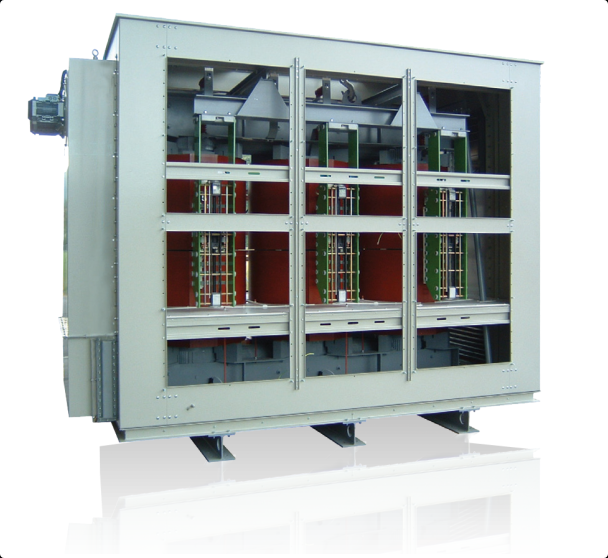
\includegraphics[width=1\linewidth]{./figs/dry-transformer.png}
	\caption{Typical air-cooled transformer with three phases $U, V, W$. The windings are the red barrel-like structures seen inside the cabinet, and the HV winding is placed within the LV winding as two concentric cylinders wrapped around the ferromagnetic core. Note that the transformer seen here is for illustrative purposes only and does not relate to this report in any way.}
	\label{fig:dry-transformer}
\end{figure}

\subsection{Case in Study} \label{sec:case-description}
For the design, training and testing of our transformer temperature model, we have a dataset provided by ABB AS \cite{abb-url}. The dataset contains operational data from a 12 MVA (mega volt-amperes) transformer as a time series stretching over the 15 months from 2018-06-04 through 2019-08-31. Sampling rates are between 1 second and 10 minutes, depending on the signal. The signals come from different sources with different quality, and the dataset therefore contains several holes where one or more signals of interest are missing.

The transformer serves an industrial process with a highly fluctuating demand, as we see in Figure \ref{fig:temp-current-aux}. It typically follows a schedule with 2 hours of service at 40-80 \% load, with 30 minute breaks in-between at no-load, as well as a 6 hours break at night-time. The cooling fans are usually turned off between the service intervals, but with a delay.

\begin{figure}[!h]
	\centering
	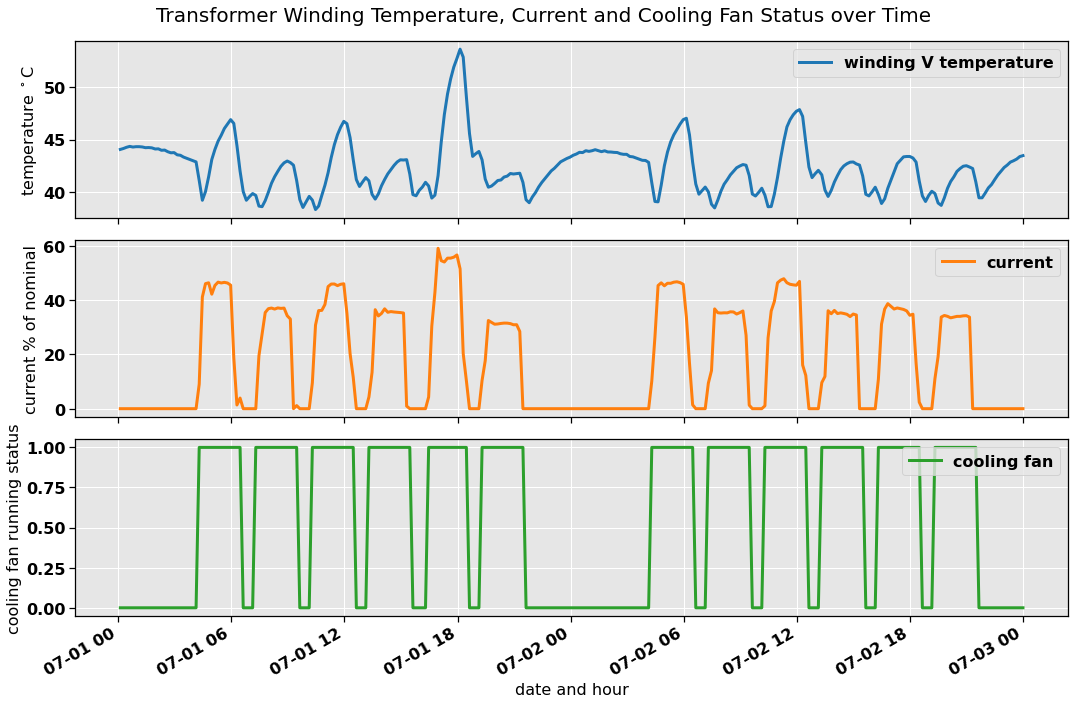
\includegraphics[width=1\linewidth]{./figs/temp-current-aux.png}
	\caption{Typical operational profile of the transformer over 48 hours. We see the winding temperature (top), the current (middle) and the running status of the cooling fans (bottom; 1 = ON, 0 = OFF). The strong temperature-dependency on current is seemingly self-evident, but the cooling fan also plays a role as we see from the increase in temperature as both current and cooling fans are turned off.}
	\label{fig:temp-current-aux}
\end{figure}

The temperature in the three phase windings should not deviate much from each other in a well-designed transformer, but there will always be small differences, as we see in Figure \ref{fig:all-winding-temperature-over-time}. The 2-4 kelvin difference is caused by some variation in the air flow through the windings due to physical location within the enclosure and different shape of the ferromagnetic core at the center of the windings. Typically, the center winding will have slightly higher temperature than the others, corresponding to the $V$ winding in Figure \ref{fig:all-winding-temperature-over-time}. Another interesting observation is that the winding temperature curve turns upwards in the time after the cooling fans are shut off. Heat is coming into the windings, probably from the HV windings (we are looking at LV temperatures). Due to the higher demands to electrical insulation and therefore more complex construction, the HV windings are not monitored.

\begin{figure}[!h]
	\centering
	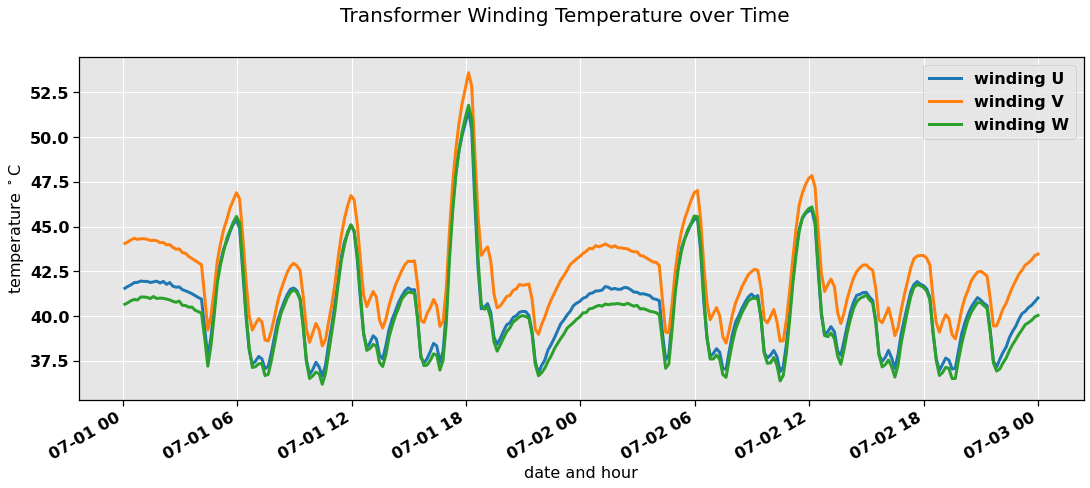
\includegraphics[width=1\linewidth]{./figs/all-winding-temperature-over-time.png}
	\caption{Development of the temperatures in windings $U,V,W$ of a healthy transformer. The temperatures follow each other closely only deviate a few degrees because of small difference in air flow through each winding.}
	\label{fig:all-winding-temperature-over-time}
\end{figure}


\section{Methods} \label{sec:methods}
% - Describe the methods and algorithms
% - You need to explain how you implemented the methods and also say something about the structure of your algorithm and present some parts of your code
% - You should plug in some calculations to demonstrate your code, such as selected runs used to validate and verify your results. The latter is extremely important!! A reader needs to understand that your code reproduces selected benchmarks and reproduces previous results, either numerical and/or well-known closed form expressions.

In the following, we will explore three different approaches for creating each of the two parts of the winding temperature model discussed in \ref{sec:transformers}; first a physical model approach where we use what we know about heat dissipation in electrical conductors along with \textit{Newton's law of cooling}; then a traditional autoregressive (AR) model approach, which will yield equations which can easily be solved by the Ordinary Least Squares (OLS) method; and lastly by using recursive neural networks (RNNs), suitable for time series data.

\subsection{First Approach: Physical Models} \label{sec:physical-model}
We will treat the two parts of our temperature model separately. First we will look at the Overall Temperature Model, which shall predict the transformer temperature based on operational parameters; then we will look at the Relative Temperature Model, which shall predict the temperature of one winding based on the temperature of the two others.

\subsubsection{Physical Model: Overall Temperature} \label{sec:physical-model-overall}
The efficiency of air-cooled transformers usually lay in the 98-99 \% range. For the 12 MVA transformer studied here, that translates to some 120-240 MW. Most of the losses are due to electrical resistance in the windings and are dissipated as heat, which must be transported out through the cooling system. The resistance is temperature dependent, and within normal operating temperatures the heat dissipation at temperature $T$ is given by
\begin{equation}
\dot{Q}_T = I^2 [R + \alpha(T - T_0)],
\end{equation}
where $I$ is the current, $R$ is the resistance at reference temperature $T_0$ (usually 20 $^\circ$C) and $\alpha$ is the temperature coefficient for the material, which is $\sim 4 \cdot 10^{-3}$ $^\circ \text{C}^{-1}$ for copper and aluminium. 

Heat is removed from the transformer through the heat exchanger according to Newton's law of cooling;
\begin{equation}
	\dot{Q}_W = uK_W (T - T_W),
\end{equation}
where $T_W$ is the water temperature, and $K_W$ is some constant representing the efficiency of heat transfer from the winding, through the air and out of the heat exchanger. The factor $u$ represents the binary \textit{ON/OFF} running status of the cooling fans -- that is; $u \in \{0,1\}$. Heat is also removed through the walls of the transformer into the room. This relation can be stated as
\begin{equation}
	\dot{Q}_A = K_A (T - T_A),
\end{equation}
where $K_A$ is similar to $K_W$, and $T_A$ is the ambient temperature. Heat transfer from the windings to the heat exchanger and the room happens at a delay, since heat is also stored in the system. If we denote the total heat capacity of the transformer by $C$, the stored heat at temperature $T$ is given by $Q_S = CT$, such that the heat flow from the windings and out of the transformer is given by the power balance
\begin{equation} \label{eq:heat-flow-compact}
	\dot{Q}_T = C \dot{T} + \dot{Q}_W + \dot{Q}_A.
\end{equation}
Since we are dealing with time series here, it is natural to approximate $\dot{T}$ by its Taylor expansion $\dot{T}_{(t)} = (T_{(t)} - T_{(t-\Delta t)})/ \Delta t$. At time $t$, Equation (\ref{eq:heat-flow-compact}) solved for temperature $T_{(t)}$ then becomes
\begin{equation} \label{eq:physical-overall}
	T_{(t)} = \frac{\frac{C}{\Delta t} T_{(t-\Delta t)} + uK_W T_W + K_A T_A + I^2 (R - \alpha T_0)}{\frac{C}{\Delta t} + uK_W + K_A - I^2 \alpha}.
\end{equation}

At this point it is tempting to let the resistance temperature coefficient $\alpha = 0$, but normal operating temperature range for a transformer is 30-130 $^\circ$C, meaning that the resistive loss in the windings will vary by $\sim 100 \cdot 4 \cdot 10^{-3} = 40 $ \%, and any accurate model would have to account for this. Further, since we do not know $T_W$ and $T_A$, neither at $t = 0$ nor later, we could maybe assume that they could be held constant. This assumption, however, is likely to not be correct, since the heat from the transformer probably will increase the room temperature as well as the incoming water temperature, which runs in a closed circuit. In addition, in order to solve this model with traditional numerical methods like the Ordinary Least Squares method to find $C, K_W, K_A$, we would have to linearize it -- which is not entirely straight-forward. We will therefore abandon this model, but the insights gained here will be useful when we design the features for our autoregressive and our neural network models.

\subsubsection{Physical Model: Relative Temperature} \label{sec:physical-model-relative}
In a healthy transformer, the temperature in any of the three windings will be closely linked to the temperature of the two others. Since the the electric impedance must be equal between the windings in order to maintain a balanced system voltage, we can assume that the electric losses will also largely be equally distributed in a well-designed transformer. Any difference in temperature is therefore likely to stem from small differences in the air flow through each winding. These assumptions correspond well with what we see in the winding temperature plots in Figure \ref{fig:all-winding-temperature-over-time}.

We will assume a linear relationship between the temperatures;
\begin{equation} \label{eq:physical-relative}
	T_X = K_{XY} T_Y + K_{XZ} T_Z,
\end{equation}
where $X,Y,Z$ may represent any one of the phase windings $U,V,W$. Given a time series with all three signals, this model can be solved easily with OLS.

\subsection{Second Approach: Autoregressive Models} \label{sec:autoregressive-model}
As for the physical in the previous section, we will make an Overall Temperature Model for the predicted temperature of the transformer based on the operation, and then a Relative Temperature Model for deviation between the windings. But first, let's take a moment to review the foundations of autoregression.

\subsubsection{A Brief Review of Autoregression} \label{sec:ar-review}
Autoregression (AR) is a statistical method made specifically for time series. It is based on the assumption that the $k$th value $y_{(k)}$ of a time series $y = \{y_{(0)}, y_{(1)}, ..., y_{(k)}, ...\}$ can be explained by a linear, weighted sum of its $p$ preceding values. Hence its name auto (self) regression. The process can be described as
\begin{equation} \label{eq:ar-basis}
	y_{(k)} = w_1 y_{(k-1)} + w_1 y_{(k-2)} + \cdots + w_p y_{(k-p)} + \varepsilon_{(k)} = \mathbf{w} \mathbf{y}_p + \varepsilon_{(k)}
\end{equation}
where the $\mathbf{w} = \{w_{i}\}$ are the weights, $\mathbf{y}_p = \{y_{(k-i)}\}_p$ are $y_{(k)}$'s $p$ preceding values, and $\varepsilon_{(k)} \sim \mathcal{N}(0,\sigma^2)$ is the process' noise. A model with $p$ terms such as Equation (\ref{eq:ar-basis}) would be referred to as a $p$th order AR model, or simply AR($p$). We can also introduce a vector of \textit{exogenous} variables $\mathbf{x}$ into this model -- that is; variables which are not decided within the system described by $y$. This model is sometimes called the ARX model and takes the form
\begin{equation} \label{eq:arx-basis}
	y_{(k)} = \mathbf{w}_y \mathbf{y}_p + \mathbf{w}_x \mathbf{x} + \varepsilon_{(k)}.
\end{equation}
Here, $\mathbf{x} = \{x_{i(k)}\}$, where $x_{i(k)}$ represents the $k$th value of the $i$th exogenous variable, and $\mathbf{w}_x = \{w_i\}_x$ are their weights. The "X" in ARX is often dropped, so the systems described in Equations (\ref{eq:ar-basis}) and (\ref{eq:arx-basis}) are both referred to as AR models. 

For the AR model to work, the time series must meet two requirements; it must be \textit{stationary} and \textit{ergodic}. Stationarity is met if the time series does not have an underlying trend, meaning that the expectation value of any two series of samples $y_1 = \{y_{(a)}, y_{(a+1)}, ..., y_{(b)}\}$, $y_2 = \{y_{(c)}, y_{(c+1)}, ..., y_{(d)}\}$ must be constant;
\begin{equation} \label{eq:stationarity}
	\mathbb{E}(y_1) = \mathbb{E}(y_2) \Rightarrow \frac{1}{b-a} \sum_{i=a}^{b} y_{(i)} = \frac{1}{c-d} \sum_{i=c}^{d} y_{(i)}.
\end{equation}
The other criteria, that of ergodicity, is met if the \textit{autocovariance} falls to zero;
\begin{equation} \label{eq:ergodicity}
	\lim\limits_{j \rightarrow \infty} \mathrm{cov}(y_{(t)}, y_{(t-j)}) = 0.
\end{equation}
Relating this to Equations (\ref{eq:ar-basis}) and (\ref{eq:arx-basis}), this means that $w_q \approx 0$ for $q > p$. Refer to \cite{shumway2017} for a thorough treatment of statistical time series analysis.

The AR model weights $\mathbf{w}_y, \mathbf{w}_x$ are then found by linear regression methods, usually OLS. To do this, we must first arrange the time series $y$ and $x_i$ in a design matrix $\mathbf{X}$ and a target vector $\mathbf{y}$ such that they can be plugged into the OLS equation for optimal weight values;
\begin{equation} \label{eq:ols}
	\hat{\mathbf{w}} = (\mathbf{X}^\intercal \mathbf{X})^{-1} \mathbf{X}^\intercal \mathbf{y},
\end{equation}
where $\hat{\mathbf{w}} = [\hat{\mathbf{w}}_y \quad \hat{\mathbf{w}}_x]^\intercal$. If we denote the length of the time series by $n$, and the number of exogenous variables $m$, $\mathbf{X}$ will be on the form
\begin{equation}
\mathbf{X} = 
	\left[ 
	\begin{array}{ccccccc}
		y_{(p-1)} & y_{(p-2)} & \cdots & y_{(0)} & x_{1(p)} & \cdots &  x_{m(p)} \\
		y_{(p)}   & y_{(p-1)} & \cdots & y_{(1)} & x_{1(p+1)} & \cdots &  x_{m(p+1)} \\	
		\vdots  & \vdots  &          & \vdots  & \vdots   &        &  \vdots   \\
		y_{(n-2)} & y_{(n-3)} & \cdots & y_{(n-p-1)} & x_{1(n-1)} & \cdots &  x_{m(n-1)} \\			
	\end{array}
\right].
\end{equation}
Thus, we will discard the first $p$ values from each time series $y, x_i$ such that  $\mathbf{y} = [y_{(p)} \quad y_{(p+1)} \quad \cdots \quad y_{(n-1)}]^\intercal$. When we solve Equation (\ref{eq:ols}), we should probably use singular value decomposition of $\mathbf{X}$ and calculate its pseudoinverse $\mathbf{X}^+$ to avoid any problems with singular matrices. See \cite{lay2016linear}.

After having found the optimal weights $\hat{\mathbf{w}}$, we will want to evaluate the model for some input time series $x_i$ of lengths $l$ and a given starting condition $y_0$. We will assume steady state initially, such that the predicted sequence $\mathbf{y}_{pred}$ becomes
\begin{equation}
\begin{aligned}
	&\mathbf{y}_{pred} = 
	\left[ 
\begin{array}{c}
	y_{(1)}	\\
	y_{(2)}	\\
	y_{(3)}	\\
	\vdots  \\
	y_{(p+2)}	\\
	\vdots  \\
	y_{(l)}	\\
\end{array}
\right]
	 \\
	&= \left[ 
		\begin{array}{ccccccc}
			y_{(0)} & y_{(0)} & \cdots & y_{(0)} & x_{1(1)} & \cdots &  x_{m(1)} \\
			y_{(1)} & y_{(0)} & \cdots & y_{(0)} & x_{1(2)} & \cdots &  x_{m(2)} \\	
			y_{(2)} & y_{(1)} & \cdots & y_{(0)} & x_{1(3)} & \cdots &  x_{m(3)} \\
			\vdots  & \vdots  &        & \vdots  & \vdots   &        &  \vdots   \\
			y_{(p+1)} & y_{(p)} & \cdots & y_{(1)}  \\
			\vdots  & \vdots  &        & \vdots     \\
			y_{(l-1)} & y_{(l-2)} & \cdots & y_{(l-p-1)} & x_{1(l)} & \cdots &  x_{m(l)} \\			
		\end{array}
	\right]
	\left[ 
\begin{array}{c}
w^{(y)}_1 \\
w^{(y)}_2 \\
\vdots \\
w^{(y)}_p \\
w^{(x)}_1 \\
\vdots \\
w^{(x)}_m \\
\end{array}
\right]	
\end{aligned}
\end{equation}
The model will thus have a run-up period of $p$ time steps, and a convergence time which depends on the system dynamics of the starting instance as well as the weights $\mathbf{w}_y$. If $y_{(0)}$ is unknown to us, we may pick a value at random or set it to zero, but the convergence time will then generally be longer. We also note that since the terms $y_{(t)}$ appear on both sides of the equation, $\mathbf{y}_{pred}$ must be calculated sequentially. 

\subsubsection{AR Model: Overall Temperature} \label{sec:ar-model-overall}
The autoregressive model encompasses a time-difference equation for the signal we want to model, and is as such a good starting point for modelling the overall transformer temperature, as shown in Equation (\ref{eq:physical-overall}). Following the discussion in Section \ref{sec:physical-model-overall}, we should expect that the exogenous variables going into the AR model in Equation (\ref{eq:arx-basis}) would be at least the current $I$ and the status of the cooling fans $u$, such that the temperature $T$ at time $t$ could be modelled as
\begin{equation} \label{eq:ar-overall-0}
	T_{(t)} = \sum_{i=1}^{p} w_i T_{(t-i)} + w_u u_{(t)} + w_{I} I_{(t)}.
\end{equation}
It would then be up to the $p$ time-difference terms to make up for the variables in Equation (\ref{eq:arx-basis}) which are not contained within $u,I$ during model fitting time -- that is; the water and room temperatures $T_W$ and $T_A$, and, importantly, any factor not captured in the physical model. The cooling fan status is binary (ON/OFF), and as we observed from the winding temperature curves in in Figure \ref{fig:temp-current-aux}, heat is flowing into the winding for some time after the transformer and the cooling fans are shut down. To account for this in Equation (\ref{eq:ar-overall-0}), we can add a term $u' = 1 - u$, such that
\begin{equation}
	w_u u_{(t)} + w'_{u} u'_{(t)} = (w_u - w'_{u})u + w'_{u},
\end{equation}
which really amounts to adding an intercept, which we will denote by $w_0$. Further, looking at the current we know that temperature is more likely to depend on the power loss in the windings, which is closer related to the current squared; $I^2$. Replacing $I$ with $I^2$ yields the equation for our AR($p$) model
\begin{equation} \label{eq:ar-overall-1}
	T_{(t)} = w_0 + \sum_{i=1}^{p} w_i T_{(t-i)} + w_u u_{(t)} + w_{I} I^2_{(t)}.
\end{equation}
The optimal weights and model order $p$ will then be determined by OLS in an iterative process.

\subsubsection{AR Model: Relative Temperature} \label{sec:ar-model-relative}
For the relative temperature model we already derived the exogenous variables in Section \ref{sec:physical-model-relative}. We will simply install the terms in Equation (\ref{eq:physical-relative}) in the general AR model in Equation (\ref{eq:arx-basis});
\begin{equation} \label{eq:ar-relative}
	T_{(t)} = \sum_{i=1}^{p} w_i T_{(t-i)} + w_X T_{X(t)} + w_Y T_{Y(t)}.
\end{equation}
Again, we expect the $p$ time-difference terms to make up for any variables not contained within the temperatures of the other windings, $T_X, T_Y$.

\subsection{Third Approach: Recurrent Neural Network Models} \label{sec:neural-model}
Before we look at how our temperature models can be implemented using RNNs, let's first give RNNs a proper introduction in the context that we will use them.

\subsubsection{A Brief Review of Recurrent Neural Networks} \label{sec:rnn-review}
Recurrent Neural Networks (RNNs) are a special class of neural networks designed for taking advantage of the time-proximity of sequential data when they make predictions. Like the simpler nodes in Feed Forward Neural Networks (FFNNs), RNN nodes sums all their inputs and adds a bias before applying an activation function like \textit{tanh}, \textit{sigmoid}, or similar. What distinguishes RNN nodes, however, is that they have a feedback loop such that the output resulting from the former input is \textit{remembered} by the node;
\begin{equation} \label{eq:rnn-node}
	\tilde{y}_{(t)} = f(w_x x_{(t)} + w_y \tilde{y}_{(t-1)} + b),
\end{equation} 
where $\tilde{y}_{(t)}$ and $x_{(t)}$ are the RNN node output and input at time $t$, $\tilde{y}_{(t-1)}$ is the node's preceding output. The learning parameters are the bias $b$ and the input and recurrent weights $w_x, w_y$. We see that the basic ingredients are the same as those for an AR(1) model studied in Section \ref{sec:autoregressive-model} (Equation (\ref{eq:arx-basis})) -- except of course for the non-linearity introduced by the activation function $f$. This non-linear relation between the time steps gives the RNN model characteristics which are very different from the linear AR model.

As for FFNNs, the bias $b$ and the input weights $w_x$ are incrementally optimized by back-propagation from output to input by using some cost function $\mathcal{C}(y, \tilde{y})$ which is evaluated on the predicted sequence $\tilde{y} = \{\tilde{y}_{(0)}, \tilde{y}_{(1)}, ...\}$ against a target sequence $y = \{y_{(0)}, y_{(1)}, ...\}$. The recurrent weight $w_y$, however, must be learned by \textit{back-propagation through time} (BPTT), once for each time step in the sequence, which makes the learning process both computationally demanding as well as at least partially sequential.

Like for FFNNs, more complex patterns can be learned by letting parallel nodes form a layer. In such a structure, the output of each layer forms a vector which is fed back into each node of the layer. This way, even more complex structures can be remembered from earlier inputs. We can also let the input be a vector, containing one or more features. Equation (\ref{eq:rnn-node}) re-written for a layer with $m$ nodes and $n$ inputs then becomes
\begin{equation} \label{eq:rnn-layer}
	\mathbf{y}_{(t)} = f(\mathbf{W}_x \mathbf{x}_{(t)} + \mathbf{W}_y \mathbf{y}_{(t-1)} + \mathbf{b}),
\end{equation} 
where we have dropped the tilde to indicate predicted values. The input, output and bias vector dimensions are $\mathbf{x} \in \mathbb{R}^{n \times 1}$, $\mathbf{y}, \mathbf{b} \in \mathbb{R}^{m \times 1}$, while the weight matrices have dimensions $\mathbf{W}_x \in \mathbb{R}^{m \times n}$ and $\mathbf{W}_y \in \mathbb{R}^{m \times m}$.

When training an RNN on a time series or a set of time series, it is most efficient to feed in \textit{mini batches} of consecutive values from the sequences at each time step. That way, the time-proximity and the amount of data that the network sees are maximized for each execution of the BPTT process, which as already mentioned is a bottleneck. With a mini batch size of $k$, the inputs and outputs thus become matrices with dimensions $\mathbf{X} \in \mathbb{R}^{n \times k}$, $\mathbf{Y} \in \mathbb{R}^{m \times k}$. We can then write Equation (\ref{eq:rnn-layer}) as
\begin{equation} \label{eq:rnn-layer-seq}
	\mathbf{Y}_{(t)} = f(\mathbf{W}_x \mathbf{X}_{(t)} + \mathbf{W}_y \mathbf{Y}_{(t-1)} + \mathbf{B}),
\end{equation} 
The dimensions of the weight matrices are as before, but the bias is now represented as a matrix $\mathbf{B} \in \mathbb{R}^{m \times k}$ with the vector $\mathbf{b}$ copied into its $k$ columns.

The next step for increasing model complexity is then to stack layers on top of each other to form a deep neural network. The network is often topped-off with a dense layer of FFNN nodes to give the model the desired output dimension (scalar, 1D, 2D, etc.). This also lets us apply some other activation function to the output than is used in the hidden RNN layers, in order to limit or expand the range if that is needed. 

The propagation of errors into the network is done as earlier -- vertically from the dense output layer towards the input layer to optimize $\mathbf{W}_x$ and $\mathbf{b}$, and horizontally by BPTT between the RNN layers. 

Further refinements to the simple RNN node with only an activation function and a feedback loop exist. They improve the node's memory both quantitatively in that memory remains stronger, and qualitatively in that the importance of new information and the memories is weighted. The most common of these is the \textit{Long Short-Term Memory} (LSTM) node, which we will use in our implementation. On the surface, they can be treated just like the simpler node described in Equation (\ref{eq:rnn-layer-seq}) -- the refinements are mostly hidden underneath the hood. We will rely on the \lstinline|tensorflow| and \lstinline|keras| Python modules for our application and not go into the details of the LSTM node here. Instead, we refer to \cite{geron2019hands} for more on advanced RNNs and their implementation.

Lastly, some words on the arrangement of input data for \lstinline|keras|. Since we will be using mini batches for the training of the RNN, we must arrange the time series in a particular data structure. The \lstinline|keras| API requires that input data is structured as a 3D \textit{tensors}. For the design matrix \lstinline|X| dimensionality is \lstinline|[n-k, k, p]|, where \lstinline|n| is the length of our time series, \lstinline|p| is the number of input features, and \lstinline|k| is the mini batch length. If we let $\mathbf{X} \in \mathbb{R}^{(n-k) \times k \times p}$ be the mathematical representation of \lstinline|X|, we must arrange the $q$th entry in the tensor \lstinline|X[q,:,:]| as
\begin{equation} \label{eq:X-tensor}
\mathbf{X}_q = 
\left[ 
	\begin{array}{cccc}
		x_{1(q)}	&x_{2(q)}	&\cdots		&x_{p(q)}	\\
		x_{1(q+1)}	&x_{2(q+1)}	&\cdots		&x_{p(q+1)}	\\
		\vdots		&\vdots		&			&\vdots		\\
		x_{1(q+k)}	&x_{2(q+k)}	&\cdots		&x_{p(q+k)}	\\
	\end{array}
\right].
\end{equation}
Likewise, if we assume that we have a target time series which is single-valued in each time step, the input target tensor \lstinline|Y| must have dimensionality \lstinline|[n-k, k, 1]|. Again, \lstinline|n| is the length of our time series and \lstinline|k| is the mini batch length. If we now let $\mathbf{Y} \in \mathbb{R}^{(n-k) \times k \times 1}$ represent \lstinline|Y|, the $q$th entry in tensor \lstinline|Y[q,:,0]| must be on the form
\begin{equation} \label{eq:Y-tensor}
Y_q = 
\left[ 
	\begin{array}{cccc}
		y_{(q)}	&x_{(q+1)}	&\cdots		&x_{(q+k)}	\\
	\end{array}
\right].
\end{equation}

Documentation on the Keras API, which is open source under the MIT license, can be found at \cite{keras-url} and. A good reference for applications with code examples is \cite{geron2019hands}.

\subsubsection{RNN Model: Overall Temperature} \label{sec:rnn-model-overall}
A lot of what we learned when we designed the features for the AR model can be reused here. We have the same two signals to work with -- phase current $I$ and cooling fan running status $u$. Even if the RNN should be able to pick up on the current-squared relationship to power loss, it does not hurt to let it know this explicitly, so we will use $I^2$ instead of $I$. This also increases variance, which is beneficial. The inverted running status $1 - u$ from the AR model is not needed, though. The bias term in the RNN nodes should be able to compensate for the all-zero input occurring when the cooling fans are shut down some minutes after the transformer goes idle.

The RNN input layer will thus be fed the two time series $u, I^2$, such that the input vector $\mathbf{x}_{(t)}$ in Equation (\ref{eq:rnn-layer}) becomes
\begin{equation}
	\mathbf{x}_{(t)} = [u_{(t)} \quad I^2_{(t)}].
\end{equation}
The output of the last layer, $\tilde{y}_{(t)}$ will then be fitted against the target scalar $y_{(t)}$ using a cost function $\mathcal{C}$. In the implementation, both $\mathbf{x}_{(t)}$ and $y_{(t)}$ must be fed into the network on the form given in Equations (\ref{eq:X-tensor}) and (\ref{eq:Y-tensor}).

The network architecture as well as hyperparameters specific to the \lstinline|keras| module generally cannot be assumed, but will be decided during training. We know, however, that since we will be feeding in mini batches during training, we will need a dense layer as the output to get the right dimensionality at the output, which will be a 1D vector for each mini batch input. The RNN layers must also be instantiated with the \lstinline|return_sequences=True| option in order to let the full mini batch sequence run through all layers. Since the mini batches are likely to be short, we can also use \lstinline|unroll=True|, which will speed up learning.

We will also have to scale the training dataset, since temperature, current squared and the binary cooling fan status are measured on wildly different scales. This also helps in the learning process, since \textit{tanh}, which is the standard activation function in \lstinline|keras| "learns best" in the $[-1,1]$ range. For this we will use the \lstinline|MinMaxScaler()| from the \lstinline|sklearn| Python module \cite{skl}, which scales each feature linearly into the $[0,1]$ range.

\subsubsection{RNN Model: Relative Temperature} \label{sec:rnn-model-relative}
As with the overall temperature model, implementation of the relative model will be quite straight-forward since we already know the features from our earlier discussions. We will use the temperatures of the two other windings as inputs to predict the temperature of the third, but in the RNN model we do not have to assume a linear relationship -- the non-linear characteristic of the neural network will account for any non-linearity in the relatinship between them. 

Using Equation (\ref{eq:physical-relative}) in Section \ref{sec:physical-model-relative} as a starting point, we get the input vector 
\begin{equation}
	\mathbf{x}_{(t)} = [T_{X(t)} \quad T_{Y(t)}].
\end{equation}
The same considerations with regards to architecture and hyperparameters apply here as they did for the overall temperature model in the previous section. We will also need to implement a dense layer as input, as well as scale the training dataset into the $[0,1]$ range.

\subsection{Data Preparation} \label{sec:data-prep}
As mentioned in Section \ref{sec:case-description}, the dataset that we have available for this report contains about 15 months of operational data for a power transformer. The time series which have been identified as relevant for developing our model are winding temperature for each individual winding on the low voltage side; the running status of the cooling fans; and all three phase currents. We do not have the ambient temperature, nor the cooling water temperature, both of which would be of interest to us.

It is safe to assume that the phase currents will be equal between the windings such that we only need to take one time series for this, which can be applied to all windings. Further, the transformer has two cooling fans, but the running status signal is common between the two.

The sampling rates differ among the time series. The currents and the cooling fan status are sampled with approximately 60 second intervals, while the temperatures are measured with 10 minute intervals. We will therefore downsample the 1 minute series to 10 minute series, which will be sufficient given the winding thermal time constant $\tau = 32$ minutes, measured by the factory during production (not referenced).

The time series also come from different sources; the currents from one, while the temperatures and cooling fan status from another. None of them are entirely reliable. The measurements may come in early or late, and the dataset contains holes of up to several weeks where one or more signals are missing, as we see in Figure \ref{fig:missing-samples}.

\begin{figure}[!h]
	\centering
	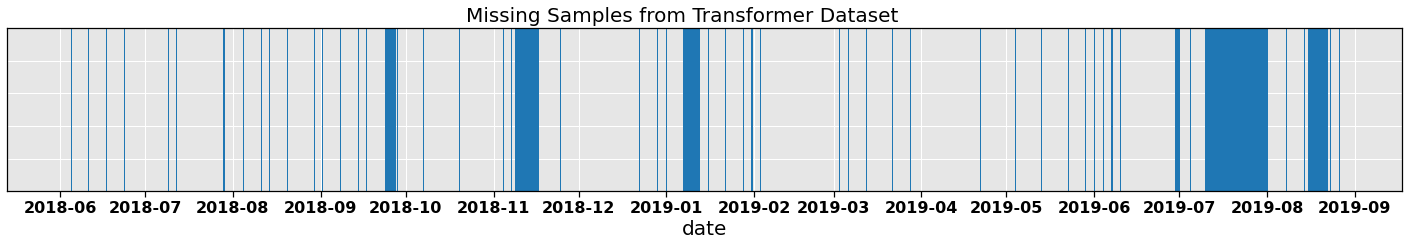
\includegraphics[width=1\linewidth]{./figs/missing-samples.png}
	\caption{Missing samples in the transformer dataset. Blue lines indicate more than one single missing sample from at least one of the time series of interest ($>25$ minutes between consecutive samples). The time series stretches over the 15 months from 2018-06-04 through 2019-08-31.}
	\label{fig:missing-samples}
\end{figure}


We saw in Figure \ref{fig:temp-current-aux} in Section \ref{sec:case-description} that the transformer operation follows a typical pattern of 2 hours service and 30 minute breaks, with a longer 6 hour break over night. In Figure \ref{fig:winding-temp-all-dataset} we see the temperature over the whole 15 month span of the dataset. Ideally, when new equipment is set into service, we should fit our model as early as possible (so-called \textit{baselining}) in order to identify changes over time relative to the new equipment. But, as we see, the transformer has an unstable period for the first half a year approximately, where the lowest temperature fluctuates between 36-38 $^\circ$C. The reason is probably that the cooling water temperature changes. 

For the overall temperature model, the unstable, first period cannot be used for model fitting since the cooling water temperature is an exogenous variable which we do not have in our model -- these are exactly the changes our model should able to identify, in that the predicted temperature will deviate from the actual. We will therefore use data from mid-November 2018 onward to fit our model.

The relative temperature model, on the other hand, is more stable since it implicitly has the information about changing external factors through the temperatures of the other windings. For fitting of this model, we will therefore be able to use data from early June 2018 already.

\begin{figure}[!h]
	\centering
	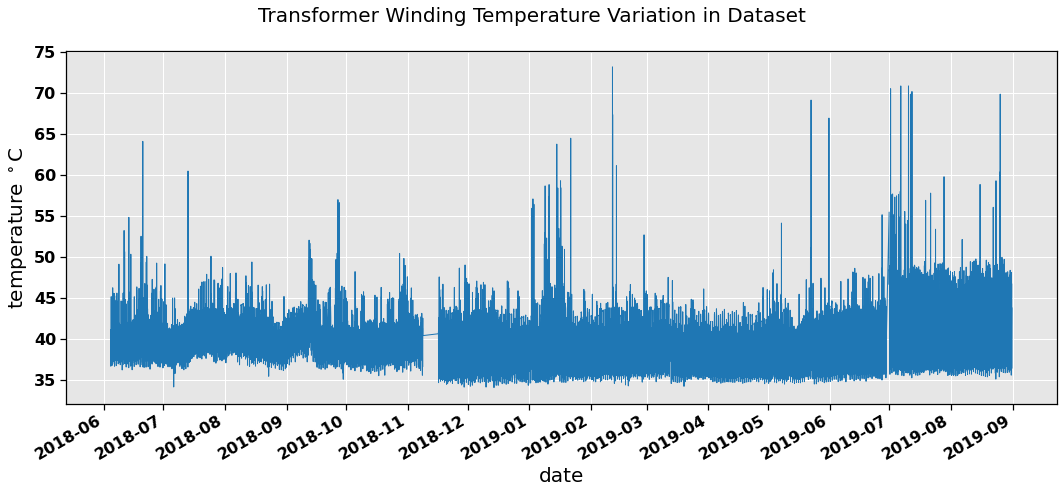
\includegraphics[width=1\linewidth]{./figs/winding-temp-all-dataset.png}
	\caption{Transformer winding temperature over the whole period of the dataset from 2018-06-04 through 2019-08-31. The transformer has an unstable period for the first six months, seen from the changing lowest temperature. We see a period of about a week with missing samples in mid-November, but note that other time series needed for the model may miss values as well.}
	\label{fig:winding-temp-all-dataset}
\end{figure}


% The first part deals with structuring and reading the data, much along the same lines as done in projects 1 and 2. Explain how the data are produced and place them in a proper context. 

% You need to include at least two central algorithms, or as an alternative explore methods from decisions tree to bagging, random forests and boosting. Explain the basics of the methods you have chosen to work with. This would be your theory part. 

% Then describe your algorithm and its implementation and tests you have performed. 

\section{Results} \label{sec:results}
% - Present your results
% - Give a critical discussion of your work and place it in the correct context.
% - Relate your work to other calculations/studies
% - An eventual reader should be able to reproduce your calculations if she/he wants to do so. All input variables should be properly explained.
% - Make sure that figures and tables should contain enough information in their captions, axis labels etc so that an eventual reader can gain a first impression of your work by studying figures and tables only.

% Then presents your results and findings, link with existing literature and more. 

We will now study the performance of our models. The section is split in two, such that we first review the overall temperature model implemented as AR and RNN; then we will look at the both implementations for the relative temperature model.

\subsection{Overall Temperature Model} \label{sec:results-overall}
As we concluded in Section \ref{sec:physical-model-overall}, we would abandon the purely physical model of the overall temperature due to its complexity and explicit reliance on the water and ambient temperatures. We will thus see results only for the AR and RNN models in this section.

For the overall model, the most interesting part of the curve fit are at the positive peaks. At the negative peaks, neither the transformer nor the cooling fans are running, and therefore we have no information to base the temperature development on other than the time lapsed since shutdown. Also, it is the function of the \textit{running} cooling system that we want to model, not the cooling curve of the idle transformer.

\subsubsection{Overall Temperature: AR Model} \label{sec:results-overall-ar}
The accuracy of the AR($p$) model which we developed in Section \ref{sec:ar-model-overall}, Equation (\ref{eq:ar-overall-1}), is shown in Figure \ref{fig:ar-model-learning} for increasing model order $p$. We see that the model quite quickly converges to an R$^2$ score above 90 \% and an MSE of around 1.3. To the right in the figure we also see that the weights $w_i$ for the time-difference terms $T_{(t-i)}$ fall towards zero. This is indicative of ergodicity in the time series (Equation (\ref{eq:ergodicity})). Along with the seeming stationarity (Equation (\ref{eq:stationarity})) observed from the temperature plot during the train and test phases in Figure \ref{fig:winding-temp-all-dataset}, the criteria for applying the AR method to this problem appear to have been met. 

Somewhat interestingly, we see that test R$^2$ is better than train R$^2$. The reason is the higher variance in the test set targets relative to the training set, at 13.3 and 8.7, respectively. The MSE, however, is better for the training set, as we would expect.

\begin{figure}[!h]
	\centering
	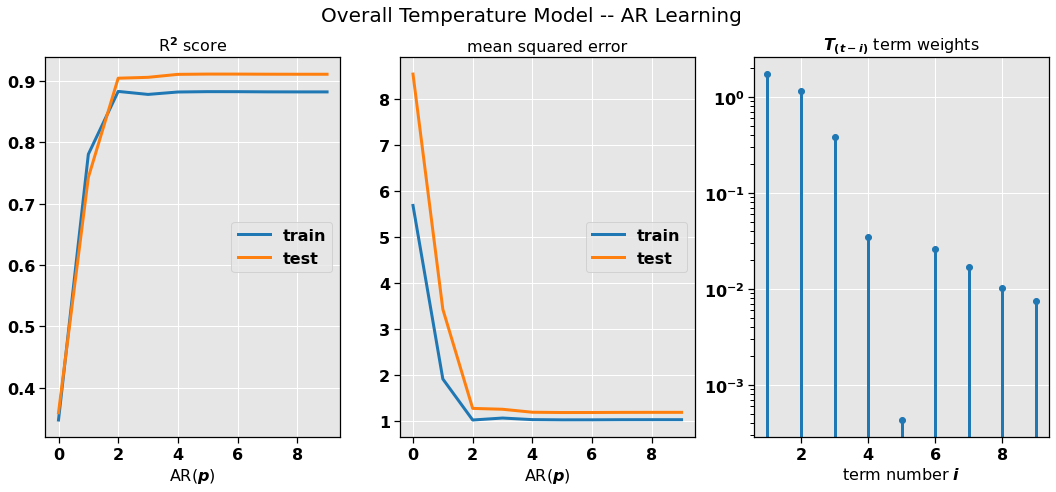
\includegraphics[width=1\linewidth]{./figs/ar-model-learning.png}
	\caption{The autoregressive AR($p$) model converges to a high R$^2$ score at around $p = 2$ already (left), also illustrated by the quickly falling MSE (center). The stem plot indicate that the AR criteria of ergodicity has been met in these time series (right). The training period stretches over about seven weeks from 2018-11-15 through 2019-01-07, while the test period stretches over the approximately two weeks from 2019-01-14 through 2019-02-01.}
	\label{fig:ar-model-learning}
\end{figure}

The high R$^2$ score and MSE indicate that the time-difference terms $p$ compensate well both for the temperature "momentum" introduced by the heat capacity of the transformer, as well as for the missing information about ambient temperature and water temperature. This is confirmed by the predicted temperature by the AR($2$) model shown in Figure \ref{fig:ar-model-performance}. This time range has been selected due to its high load variability, and we see that the model predicts the positive peaks with only around 1 K error. The error is larger in the prediction of the negative peaks, which occur as the transformer is shut off, and hence is not critical. Increasing the model order $p$ improves on this, but comes at a cost to accuracy in the positive peaks.

We also see that the prediction for the over-night breaks is quite poor -- the model tries to predict the average value in order to satisfy the OLS cost function. This error can be disregarded completely since the model receives no information during this time ($I^2, u = 0$).

\begin{figure}[!h]
	\centering
	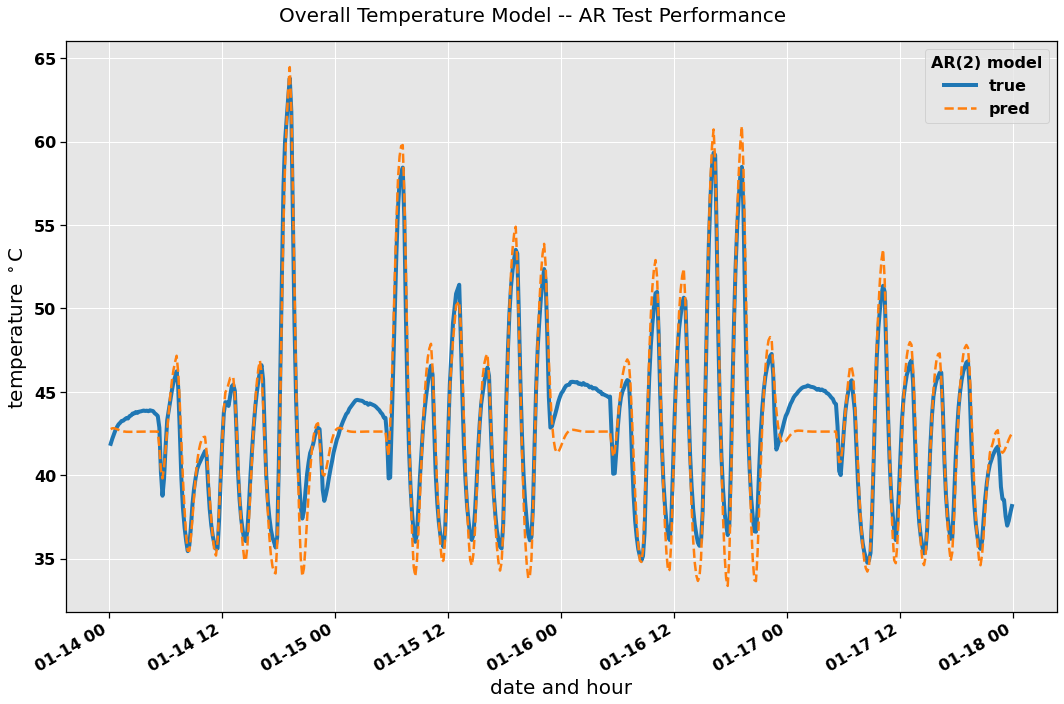
\includegraphics[width=1\linewidth]{./figs/ar-model-performance.png}
	\caption{The AR($2$) model during a time range with highly varying demand. Performance is good, especially while the transformer is in service. During the $\sim 30$ minute breaks (negative peaks) and night performance is poorer, but this is not critical.}
	\label{fig:ar-model-performance}
\end{figure}

The coefficients in the overall AR(2) model for each winding $U,V,W$ are on a per-unit input basis are
\begin{equation}
\begin{aligned}
	T_{U(t)} &= 5.2 + 1.5T_{U(t-1)} - 0.60T_{U(t-2)}- 0.90u + 1.4I^2 \cdot 10^{-5} \\
	T_{V(t)} &= 5.0 + 1.5T_{V(t-1)} - 0.61T_{V(t-2)}- 0.97u + 1.4I^2 \cdot 10^{-5} \\
	T_{W(t)} &= 5.1 + 1.5T_{W(t-1)} - 0.61T_{W(t-2)}- 0.86u + 1.4I^2 \cdot 10^{-5} \\
\end{aligned}.
\end{equation}
The temperatures typically lay within the 30-100 $^\circ$C range; $u$ is either 0 or 1; and the nominal current squared $I^2 = 3.97 \cdot 10^5$ A$^2$.

\subsubsection{Overall Temperature: RNN Model} \label{sec:results-overall-rnn}
The overall temperature RNN model has been implemented as a two-layer LSTM network with a dense output layer of FFNN nodes. The input layer has 30 nodes, the hidden RNN layer 18 nodes and the output layer has nodes corresponding to the length of the mini batch. 

The network has been implemented in \lstinline|keras| and stacked using \lstinline|Sequential()|. Initially, the network had somewhat poor responsiveness to changing $I^2$, but by trial and error, good performance was achieved by damping the feedback by using \lstinline|recurrent_dropout=.5| and input \lstinline|dropout=.0|, then \lstinline|compile()| with \lstinline|optimizer='adam'| and \lstinline|loss='mse'|. Further, model fitting was done using \lstinline|Sequential.fit()|, with \lstinline|epochs=50| and stochastic gradient descent \lstinline|batch_size=50|.

The mini batch size was found to be an important hyperparameter. In Figure \ref{fig:rnn-model-learning} we see the increasing accuracy of the model as the batch size grows. It reaches approximately the same R$^2$ score and MSE as the AR model. 

\begin{figure}[!h]
	\centering
	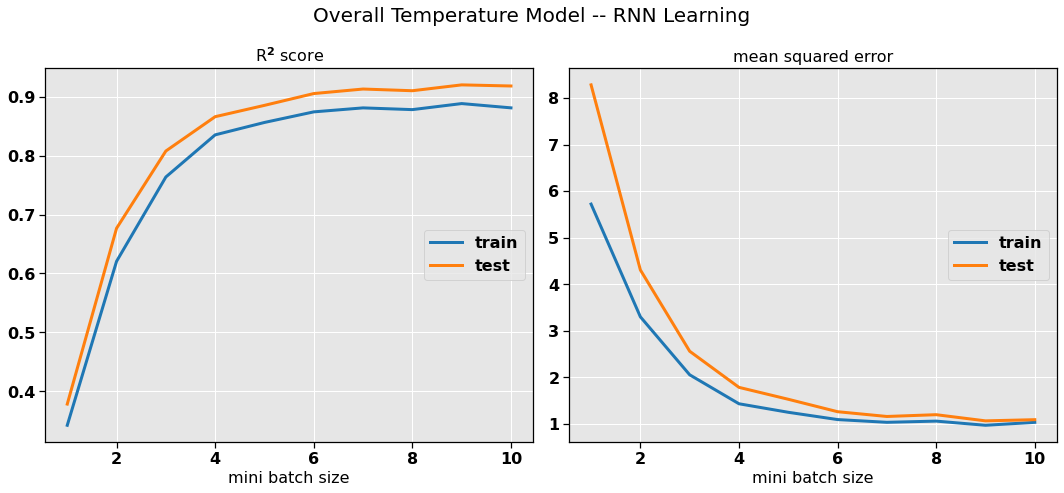
\includegraphics[width=1\linewidth]{./figs/rnn-model-learning.png}
	\caption{The recurrent neural network model converges to a high R$^2$ score with mini batch size 6 already (left), also illustrated by the quickly falling MSE (right). The training period stretches over approximately seven weeks from 2018-11-15 through 2019-01-07, while the test period stretches over the approximately two weeks from 2019-01-14 through 2019-02-01.}
	\label{fig:rnn-model-learning}
\end{figure}

The RNN was trained on the same data as the AR model, but the AR model would achieve a better result on a smaller dataset than would the RNN model. Thus, the RNN model is more data hungry than the other. In Figure \ref{fig:rnn-model-performance} we see the RNN model's performance in the same time range as was shown for the AR model in Figure \ref{fig:ar-model-performance}. The RNN predicts both directions with high accuracy, and we only have the occasional overshoot, like 1-2 K overshoot in the evening on 2018-01-17. On the positive peaks, accuracy is similar to the AR model, if maybe a little over the top where the AR is a little under the top, but the margins are really small here. On the negative peaks, where both the transformer and the cooling are off, prediction is better for the RNN model. It seemingly knows how deep temperature will go given its former load. However, exact prediction of the negative peaks is not critical, since it is the cooling system performance which we are interested in.

As with AR, the RNN also tries to average the night breaks. The LSTM memory seemingly is not good enough to remember across the $\sim 60$ sample span when both inputs $I^2$ and $u$ are zero. This can be compensated by increasing the batch size, but comes at a cost to learning efficiency and is anyways not needed for the utility of the model.

\begin{figure}[!h]
	\centering
	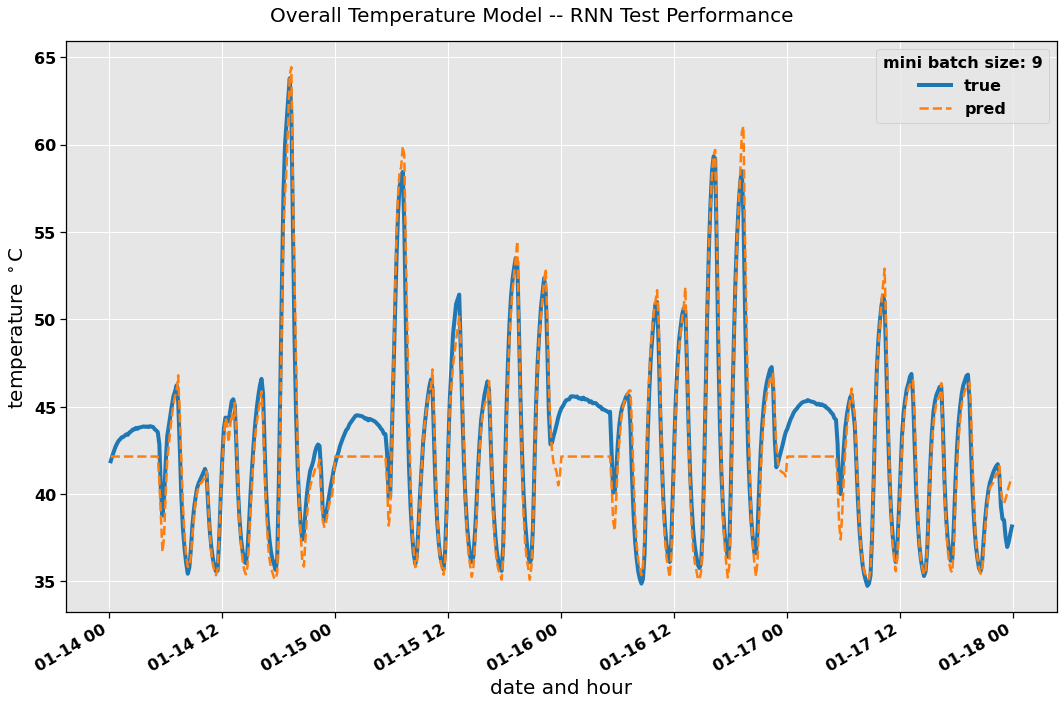
\includegraphics[width=1\linewidth]{./figs/rnn-model-performance.png}
	\caption{The RNN model during the same time range as seen for the AR model in Figure \ref{fig:ar-model-performance}. The RNN predicts accurately both positive and negative peaks. Mini batch size is 9 in this model.}
	\label{fig:rnn-model-performance}
\end{figure}

\subsection{Relative Temperature Model} \label{sec:results-relative}
In Section \ref{sec:physical-model} we showed how three models for the relative temperature could be made -- by OLS using the temperature of two windings to predict the third; as an AR($p$) model, which would then be solved by OLS; and as an RNN. Since the pure OLS model correspond exactly to the AR($0$) model, we will treat this as a special case of the AR model in the following discussion.

\subsubsection{Relative Temperature: AR Model} \label{sec:results-relative-ar}
Our assumption about the linear relationship between the winding temperatures in Section \ref{sec:physical-model-relative}, Equation (\ref{eq:physical-relative}), seems to have been correct. In Figure \ref{fig:ar-model-learning-relative} we see that we reach a very high R$^2$ score and low MSE with AR($0$) already. Any improvement achieved by introducing the time-difference terms can only have very little impact on the quality of the result, as we see in Figure \ref{fig:ar-model-performance-relative} -- the match is almost perfect, with only minor overshoot of about 1 K on the highest positive peaks. Thus, OLS with the physical approach has the best approximation for the relative model. Note also that this result was achieved with only a single day's data for training, which really matters in a practical application.

As for the overall temperature model, we give the coefficients in the relative AR(0) model for each winding $U,V,W$ on a per-unit input basis;
\begin{equation}
\begin{aligned}
T_{U(t)} &= 0.23T_{V(t)} + 0.75T_{W(t)} \\
T_{V(t)} &= -1.4T_{W(t)} + 2.5T_{U(t)} \\
T_{W(t)} &= 1.2T_{U(t)} - 0.22T_{V(t)} \\
\end{aligned}.
\end{equation}

\begin{figure}[!h]
	\centering
	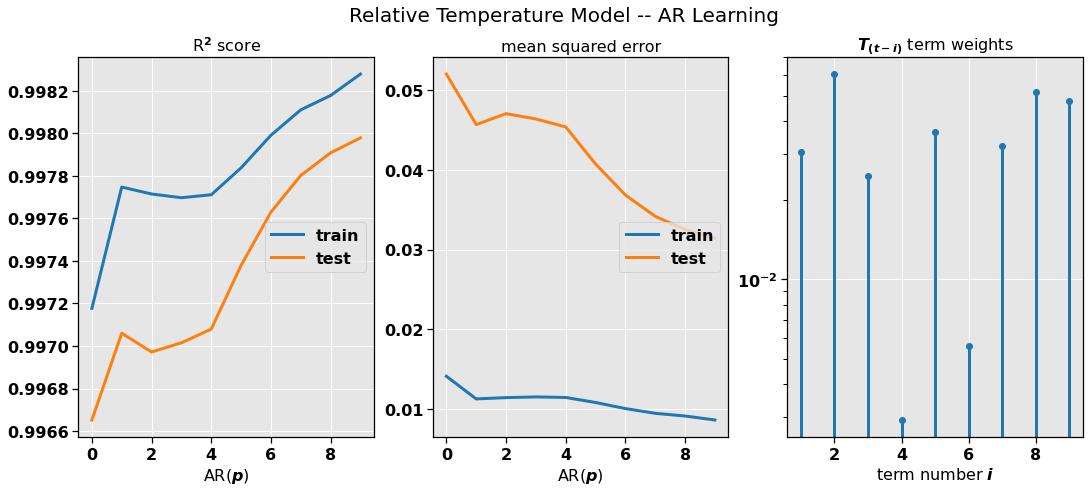
\includegraphics[width=1\linewidth]{./figs/ar-model-learning-relative.png}
	\caption{The autoregressive AR($p$) model converges to a very high R$^2$ score at around $p = 0$ already (left), with only minor improvement beyond that point. For higher orders, we see from the stem plot (right) that the model balances the weights on the time-difference terms against that of the other winding temperatures, but the result is largely unchanged. The training period stretches over one day only; from 2018-06-05 at midnight until 2018-06-06 at midnight, while the test period stretches over the approximately two weeks from 2019-01-14 through 2019-02-01, as in the results from the previous section.}
	\label{fig:ar-model-learning-relative}
\end{figure}

\begin{figure}[!h]
	\centering
	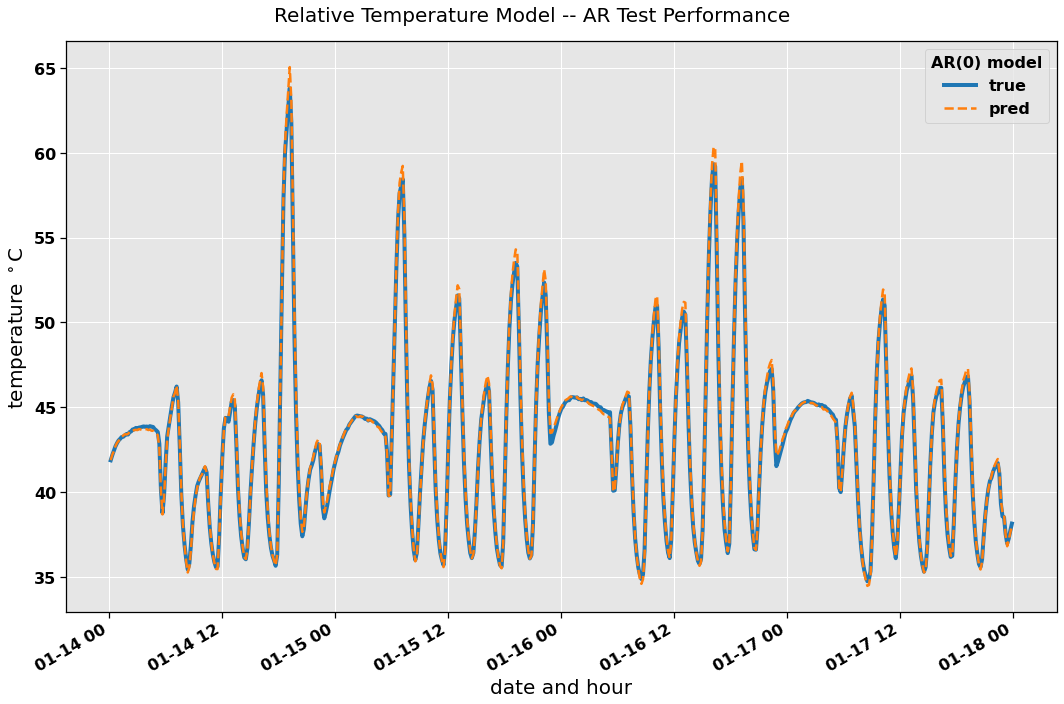
\includegraphics[width=1\linewidth]{./figs/ar-model-performance-relative.png}
	\caption{The AR($0$) or physical relative temperature model during a time range with highly varying demand. The model achieves an almost perfect match, both during when the transformer is in service and when idle.}
	\label{fig:ar-model-performance-relative}
\end{figure}



%\clearpage
\subsubsection{Relative Temperature: RNN Model} \label{sec:results-relative-rnn}
The RNN for the relative model can be simplified considerably compared to the overall model. Figuring out the linear relationship that we saw in the previous section between the two features in the design matrix and the target is a much simpler problem than the former, which had a time-difference dependency. We will use a network with only one RNN layer containing 5 nodes, in addition to the dense FFNN output layer. Other hyperparameters could be kept the same as in Section \ref{sec:results-overall-rnn}. 

Figure \ref{fig:rnn-model-learning-relative} shows again the progressive accuracy of the model as we increase the mini batch size while keeping the number of epochs constant. To the left we see that the model reaches a R$^2$ score of about 0.75 at about size 4 and then climbs steadily upwards towards approximately 0.85 at batch size 10. This is a quite good approximation, but of course much worse than the AR($0$) model we found above in the previous section, which approached 1.0. 

The curve fit of the RNN model is quite good, with proper prediction within 2-3 K error except for the highest peaks, as we see in Figure \ref{fig:rnn-model-performance-relative}. However, considering the relative simplicity of the problem, the result is somewhat disappointing. The model was trained on one month of data.

\begin{figure}[!h]
	\centering
	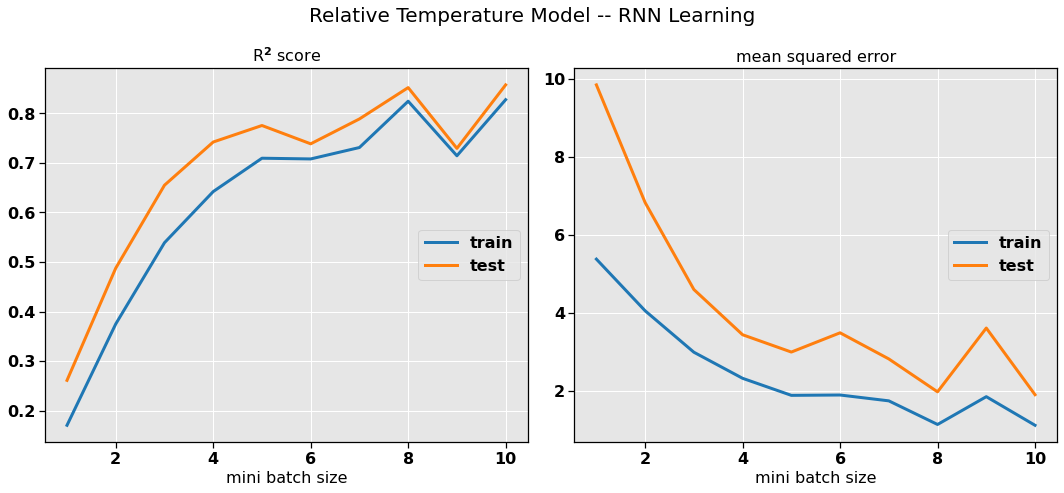
\includegraphics[width=1\linewidth]{./figs/rnn-model-learning-relative.png}
	\caption{The recurrent neural network model reaches an R$^2$ score of approximately 0.85 with mini batch size 10 (left). The training period stretches over one month from 2018-06-04 through 2018-06-04, while the test period stretches over the same two weeks as earlier -- from 2019-01-14 through 2019-02-01.}
	\label{fig:rnn-model-learning-relative}
\end{figure}

\begin{figure}[!h]
	\centering
	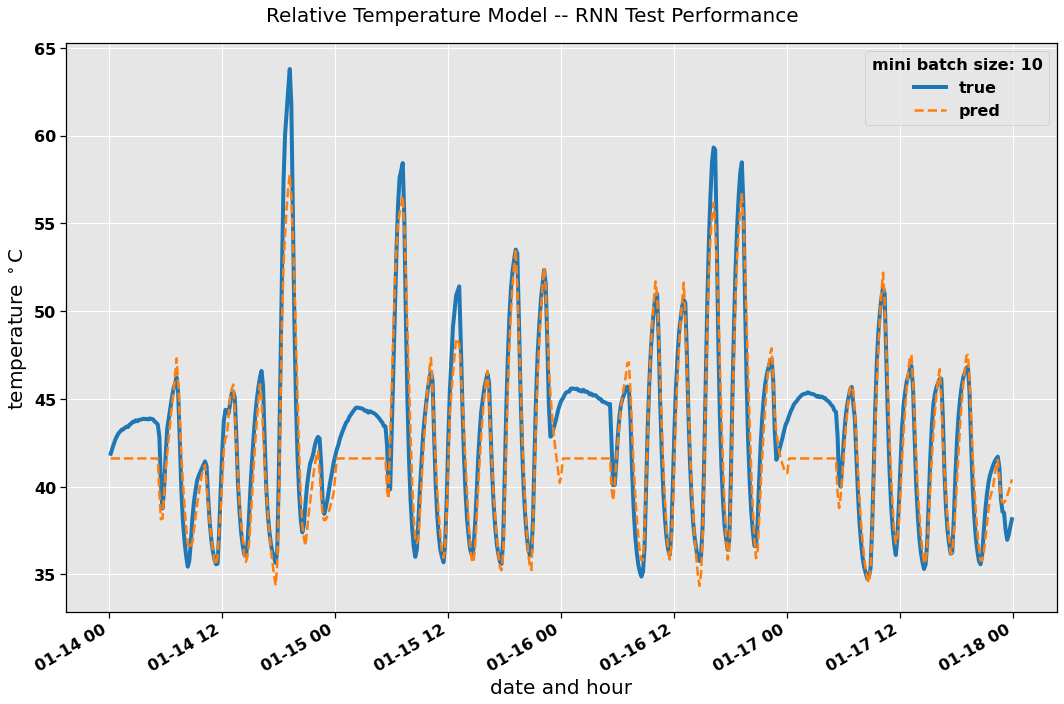
\includegraphics[width=1\linewidth]{./figs/rnn-model-performance-relative.png}
	\caption{The RNN model does not perform poorly, but compared to the AR(0) model seen in Figure \ref{fig:ar-model-performance-relative}, it cannot compete. The RNN predicts accurately both positive and negative peaks with a few degrees error. Mini batch size is 10 in this model.}
	\label{fig:rnn-model-performance-relative}
\end{figure}

\clearpage
\section{Discussion and Conclusion} \label{sec:conclusion}
% - State your main findings and interpretations
% - Try as far as possible to present perspectives for future work
% - Try to discuss the pros and cons of the methods and possible improvements

% Finally, here you should present a critical assessment of the methods you have studied and link your results with the existing literature. 
We have seen that by using only current, cooling fan running status and winding temperatures -- measurements which are normally collected and logged in an industrial application -- we can create a precise model of the transformer's cooling system. The model correctly predicts the transformer winding temperature under dynamic operation -- either as an overall temperature based on current and cooling fan running status; or it predicts the relative temperature of each of the three windings, based on the temperature of the others. The model predicts the temperatures with high reliability, and only deviate around 1 K at the highest load peaks.

The model requires no parametrization. Model creation is also completely non-intrusive in that it requires no specific load patterns for baselining of the transformer -- something which in many cases would be impractical or even impossible in an industrial application. In the case of the relative winding temperature model, only a single day's data is required. The overall winding temperature model needs some 6-8 weeks of data. Sampling rate may be as little as every 10 minutes.

The two parts of the model are made as a purely linear combination of the winding temperatures in the case of the relative temperature, while the overall may use either an autoregressive method or a more advanced recurrent neural network. 

In a practical application, simplicity really matters, and the most valuable part of the model is therefore the relative winding temperature model, which has an R$^2$ score above 99 \%, requires very little data to fit, and is simple to implement. Compared to this, any competing model would perform badly, and even with an R$^2$ well above 80 \%, the RNN remains unsuitable. If it were necessary, it should be possible to implement this model as a simple FFNN with only a few nodes, since there really is no time-dependence in the linear model.

The same considerations regarding simplicity goes for the overall winding temperature model as well. Even though performance was slightly better for the RNN, the AR model is simple to implement for instance in an industrial programmable logic controller, which has limited computing resources and often only very basic software libraries. On the other hand, if the implementation would be on a server running a cloud environment, which may often be the case, those considerations are not as important. Still, we have seen that the RNN is more data hungry than the simpler linear methods, which also have the added benefit of providing a model which describes its dependency on its variables and is understandable to the human.

Future work, in addition to final validation through tests in a lab or in the field, would be to expand the model to include other measurements like water temperature and air temperature into and out of the transformer's heat exchanger in applications where those measurements would be available. These improvements would make the model able to spot specific problems under development, like oxidation in a heat exchanger, in a completely non-intrusive way. Further, the model suggested here is easily transferred to other electric machines like motors or generators, which have their own particular fault modes relating to their cooling systems.


%\clearpage
%\vspace{5mm}

%\clearpage
\bibliographystyle{unsrt}
\bibliography{project3.bib}
\end{document}
